\documentclass{beamer}
\usepackage[utf8]{inputenc}
\usepackage{xcolor}
\usepackage{graphicx}

%\usetheme{metropolis}
\usetheme{metropolis}

\title{Estimating the number of COVID-19 victims by using a Monte Carlo
algorithm on a generalized logistic equation}

\author{Biagio Paparella}
\institute{Oberseminar - Institute for Numerical Simulation - Bonn}
\date{10.06.2020}

\begin{document}
\frame{\titlepage}

\begin{frame}
	\frametitle{Introduction and motivation}

	Goal of my recent work: influenced by recent events,
	try predicting the number of COVID-19 victims.

	\begin{itemize}
\item <1-> (Possibly) the most reliable measurement, compare e.g. with infected
	(test problems, etc...);
\item <2-> Studied time span: April to predict May (stable conditions);
\item <3-> Idea: if it works, repeat now to predict June/July...
\item <4-> Chosen Countries: Germany, France, Italy.
	\end{itemize}


\end{frame}

\begin{frame}
	\frametitle{The model in theory: ODE description}
	$X(t)$ : number of deaths in time. Modeled via 
	a simple 1-d ODE with initial conditions $X_0$. 
	Generalized logistic map 
	(S-shaped, exp initially, then flat):
		\begin{equation}
			X'(t) = \frac{\color{red}{\color{red}{q}}}
			{\color{red}{v}} X(t)
			\left ( 1 - \left( \frac{X(t)}{\color{red}{Q}} \right)^
			{\color{red}{v}}\right )
\end{equation}

	\begin{itemize}
		\item<1-> It has a close form solution (here not written);
		\item<2-> Depends on the parameter 
			$P = \{\textcolor{red}{q}, 
				\textcolor{red}{Q}, 
				\textcolor{red}{v}\}$
			(more next slide). 
	\item<3-> In others words: assume $\exists P \in \mathbb{R}^3$,
		s.t. $X^P(t)$ correctly describe the (past and future) 
			number of victims. Want to find $P$.
	\end{itemize}
\end{frame}

\begin{frame}
	\frametitle{The model in theory: parameters description}
	Do not need to remember the form of $X^P(t)$. It's worth 
	understanding the role of the parameter $P$.
	\begin{itemize}
		\item $P = \{ q, Q, v \}$ are all \emph{strictly} positive.
		\item <2->$Q$ is the carrying capacity 
			($\lim_{t \to \infty} X(t) = Q$);
		\item <3-> $v =1$ gives the \emph{simple} logistic model,
			while $v \to 0^{+}$ the \emph{Gompertz} model. Both
			very famous and used in the literature;
		\item <5-> $q$ is related to the "starting" exponential
			growth;
	\end{itemize}

	\begin{itemize}
		\item<6->
			\textcolor{orange}{Intuition}: 
			$Q$ the "final" number of victims
	($10, 30, 50K$?), we expect $0 < q << 1$
	(warning: this comes from the simple logistic)
	and we prefer
	$0 < v < 1$ oscillating between the two common models
	(but no actual math. restriction).

\item<7-> Keep in mind: 
	$Q$ large, $>10.000$, $v$, $q$ small, $\in [0,1]$.
	\end{itemize}

\end{frame}

\begin{frame}
	\frametitle{The model in practice: observed vector}
	The available dataset are "numbers of total deaths until day $t_i$":
	discrete, limited, ODE trajectory of $X^P_{X_0}(t)$.
	\textcolor{blue}{Use them to infer $P$}.

	\begin{block}{}
	Fix $T+1$ times $\{t_i\}_{i = 0,\dots, T}$, e.g. 21 days.
		The \textcolor{olive}{observed vector} 
		$\textbf{y} \in \mathbb{R}^{T+1}$
        is the random variable defined componentwise as:
	\begin{equation}
        	y_i(\omega) = X^P_{X_0} (t_i) + \eta_i(\omega)
	\end{equation}
		where $\eta_i \sim \mathcal{N}(0, \sigma^2_i)$, $i \in \{0,
		\dots,T\}$.
	\end{block}

	\begin{itemize}
		\item<2->
	In other words, $\textbf{y}$ is what we measure: "noised truth".
	\end{itemize}
\end{frame}

\begin{frame}{The model in practice: noise}
	To assume an error of the form
	\begin{equation}
		y_i(\omega) = X^P_{X_0} (t_i) + \eta_i(\omega)
	\end{equation}
	is a \textcolor{red}{strong} assumption (I know). Need to decide 
	the standard variations $\sigma_i$ for each day. Abritrately.


	Quantile formula:
	$\eta_i \sim N(0, \sigma_i^2) \implies
\mathbb{P}[ - 2 \sigma_i \leq \eta_i \leq 2 \sigma_i] \geq 95\%$


	Read like: "trust $0 \pm 2 \sigma_i$". Adding the real
	number $y_i$: "trust $y_i \pm 2 \sigma_i$. So 
	we arbitrarily choose:
	\begin{itemize}
		\item <2-> \textcolor{olive}{Case 1}: 
			$\sigma_i$ s.t. we trust
		$y_i \pm \frac{y_i}{10}$, i.e. "$10\%$ of error";
	\item <3-> \textcolor{magenta}{Case 2}: $\sigma_i$ s.t. we trust
		$y_i \pm y_i$, i.e. "$100\%$ of error";
	\item <4-> \textcolor{red}{Warning}:
		the inference algorithm [not yet described]
		is destroyed for higher errors, but not with our cases
			- checked with toy model data.
	\end{itemize}
\end{frame}


\begin{frame}
	\frametitle{Inference technique: MCMC}
	\begin{itemize}
		\item<1->
	We have the model $X^P(t)$, the noise structure and the data.
	Last step: choose how to infer $P \in \mathbb{R}^3$.


	\item<2-> in general, I am mainly into the topic
		"Bayesian Inverse Problems", where a 
		common technique is the "Preconditioned Monte Carlo" algorithm
			(pCN);

	\item<3-> most suitable for infinite-dimensional cases,
		large data, inversion of PDEs...

	\item<4-> here: only $20$ days, $3$ real parameters, a simple
		1-dim ODE with close form solution. 

	\item<5-> But I was curious and insisted: let's use the 
		pCN algorithm anyway!

	\item<6-> \textcolor{blue}{In brief}: we infer $P$ by using
		a Monte Carlo algorithm.

	\end{itemize}
\end{frame}

\begin{frame}
	\frametitle{The Bayesian setting: how to infer $P$?}

	\begin{itemize}
		\item<1-> The idea is: \emph{given} the data $\textbf{y}$,
			find $P$. Equivalent: find
			$\mathbb{P}[P | \textbf{y}]$.
		\item<2-> Step 1: assume to have a probability
			density on $\mathbb{R}^3$, called the
			\textcolor{blue}{prior}. Blind guess about $P$,
			i.e. $\mathbb{P}[P \in dx]$.
			(more later);

		\item<3-> Step 2: interpret the read data as
			$\mathbb{P}[\textbf{y} | P]$
			(\textcolor{magenta}{likelihood}, 
			obtain a complete formula
			by using the Gaussian noise, etc...)

		\item<4-> Step 3: conclude by using the Bayes formula:
			\begin{equation}
				\mathbb{P}[P | \textbf{y}] \propto
				\mathbb{P}[\textbf{y} | P] 
				\times \mathbb{P}[P]
			\end{equation}
			where $\mathbb{P}[P | \textbf{y}]$ is the
			\textcolor{olive}{posterior} measure.

		\item<5-> In brief: fix a belief about $P$, i.e. the prior. 
			Read the data, obtain the likelihood.
			Multiply them to have the posterior
			probability, containing 
			information about the "true" $P$
			given the data (details omitted on purpose).
		\item<6-> \textbf{Infer $P$ = sample from the posterior}
	\end{itemize}
\end{frame}

\begin{frame}
	\frametitle{The pCN Monte Carlo method}
	Let $\mathbb{P}[P | \textbf{y}]$ be the posterior on $\mathbb{R}^3$.
	Let $0 < \beta < 1$ the speed parameter, and the acceptance
	probability, for $v, u \in \mathbb{R}^3$:
	\begin{equation}
		a(u, v) \doteq \min \{ 1, \frac{ \mathbb{P}(\textbf{y} | v )}
                                {\mathbb{P}(\textbf{y} | u)} \}
	\end{equation}
	To produce a \textbf{single sample}, construct a chain
	$\{ x_i \} _{i \in \mathbb{N} }$ as follows:

\begin{enumerate}
        \item set $x_0 \in \mathbb{R}^n$ \textbf{arbitrarily}. Then, for each
                $k > 0$:
        \item sample a point $R \in \mathbb{R}^3$
		from the \textbf{gaussian} prior $\mathbb{P}(P \in dx)$;

        \item  propose a candidate as
                $
                \hat{x}_{k} = \sqrt{(1 - \beta^2)} x_{k-1}
                        + \beta R
                $;
        \item   accept it (i.e. set $x_{k} = \hat{x}_{k}$)
                with probability $a(x_{k-1}, \hat{x}_k)$;
        \item (accepted or not) repeat from 2;
\end{enumerate}

	Run $120.000$ multiple chains in parallel, different starting point, 
	each stopped after $250.000$ iterations. Beta around $0.05$, s.t.
	acceptance rate $\sim 25\%$. 
	\textcolor{olive}{Last missing info: which prior?}
\end{frame}


\begin{frame}
	\frametitle{Prior measure on $P$: part 1}
	Before moving to the numerical results, we need to clarify the
	structure of the prior measure. It influences the results.
	\begin{itemize}
		\item <1-> The pCN Monte Carlo algorithm \emph{requires}
			a centered Gaussian prior (on $\mathbb{R}^3$).
		\item <2-> Problematic: $P \in \mathbb{R}^3$ 
			is strictly positive...so
			we just rejected the negative proposals...(pitfall?)...
		\item<3-> and we assumed a prior structure with covariance
			matrix
			\begin{equation}
				\begin{pmatrix}
			        \sigma_q^2 & 0 & 0 \\
    				    0 & \sigma_Q^2 & 0 \\
     				   0 & 0 & \sigma_v^2
			\end{pmatrix}
			\end{equation}
		\item <4-> Therefore: we only need to choose the $\sigma$,
			and then we can move on the simulations!
	\end{itemize}
\end{frame}


\begin{frame}
	\frametitle{Prior measure on $P$: part 2}
	Goal of this slide: explain how the values for $\sigma_q$, $\sigma_Q$
	and $\sigma_v$ have been chosen.
	\begin{itemize}
		\item <1-> The idea is: the prior represents the "guess", the
			"default" choice. But if "nothing is done", the
			phenomenon propagates exponentially.
			Therefore we run an exponential interpolation,
			and register the number of victims
			in 1 Month: $K$. Then choose 
			\textcolor{blue}{$\sigma_Q$} in order
			to have the Gaussian $95\%$  quantile just 
			below this quantity;
		\item <2-> Dealing with 
			\textcolor{blue}{$\sigma_q$} and 
			\textcolor{blue}{$\sigma_v$}, they have 
			been chosen in order to have that quantile between
			$0$ and $1$.
		\item <3-> These idea formalize the intuition
			that we expect parameters in these range,
			without \emph{forcing} any constraint.
	\end{itemize}
\end{frame}

\begin{frame}
	\frametitle{How to read the results}
	\begin{itemize}
		\item<1-> Now all the parameters, assumptions, hypothesis
			should be clear. In particular,
			we are using a possibly-not-so-good
			Monte Carlo algorithm with strong assumptions
			on the noise and the prior;
		\item <2-> We remark: 
			by reading the data we infer a 3-dimensional
			probability measure for $P$...
		\item<3-> we clustered it by the k-means algorithm 
			and selected three set of parameters:
		\item <4-> the \textcolor{red}{worst} case, i.e.the triple
			with the highest
			value for $Q$; the \textcolor{brown}{best} 
			(converse) and the
			\textcolor{violet}{expectation}.
		\item <5-> We have plots for the "10\%" error scenario,
			as well as for the "100\%" (\emph{meaning
			explained before})
	\end{itemize}
\end{frame}

\begin{frame}
	\frametitle{Results: Italy, assuming $10\%$ of "error"}
	\begin{figure}
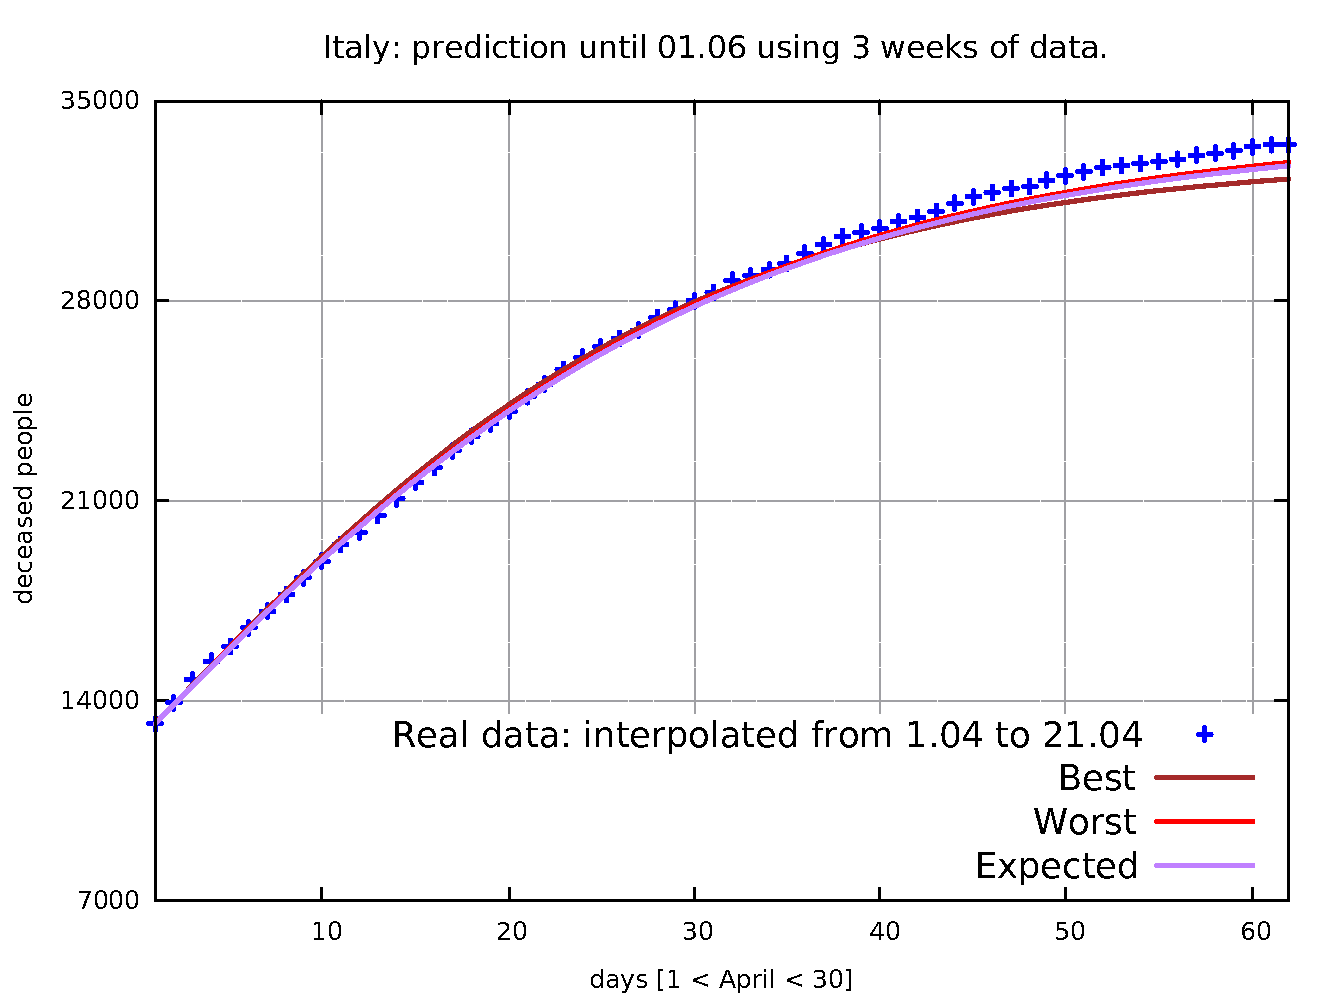
\includegraphics[width=\linewidth]{../../err10p_simulations/it/1-21/1-21.pdf}
	\end{figure}
\end{frame}

\begin{frame}
	\frametitle{Results: France, assuming $10\%$ of "error"}
	\begin{figure}
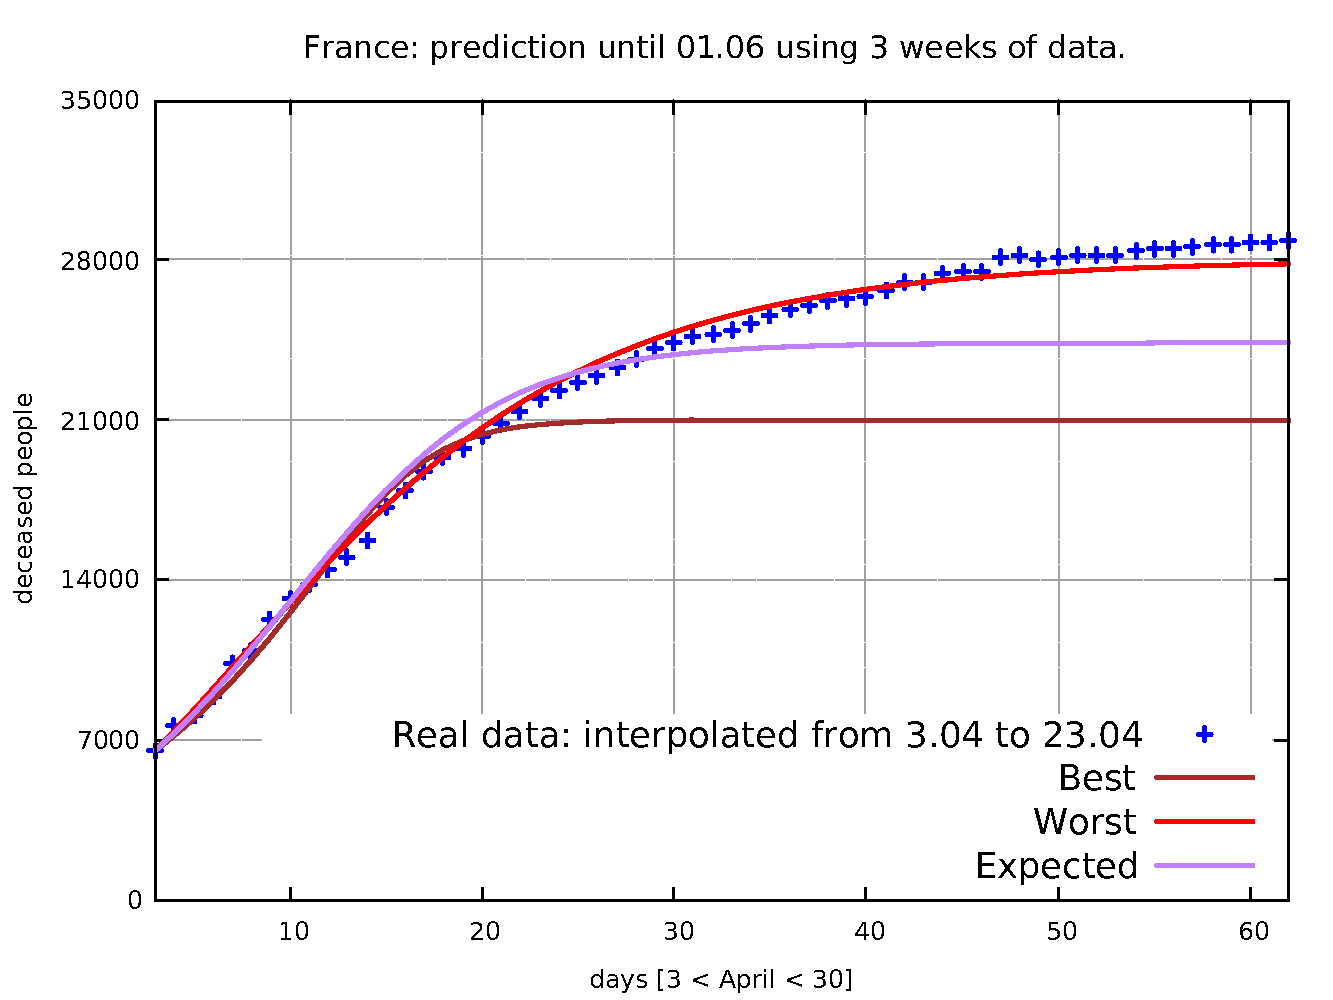
\includegraphics[width=\linewidth]{../../err10p_simulations/fr/3-23/3-23.pdf}
	\end{figure}
\end{frame}

\begin{frame}
	\frametitle{Results: Germany, assuming $10\%$ of "error"}
	\begin{figure}
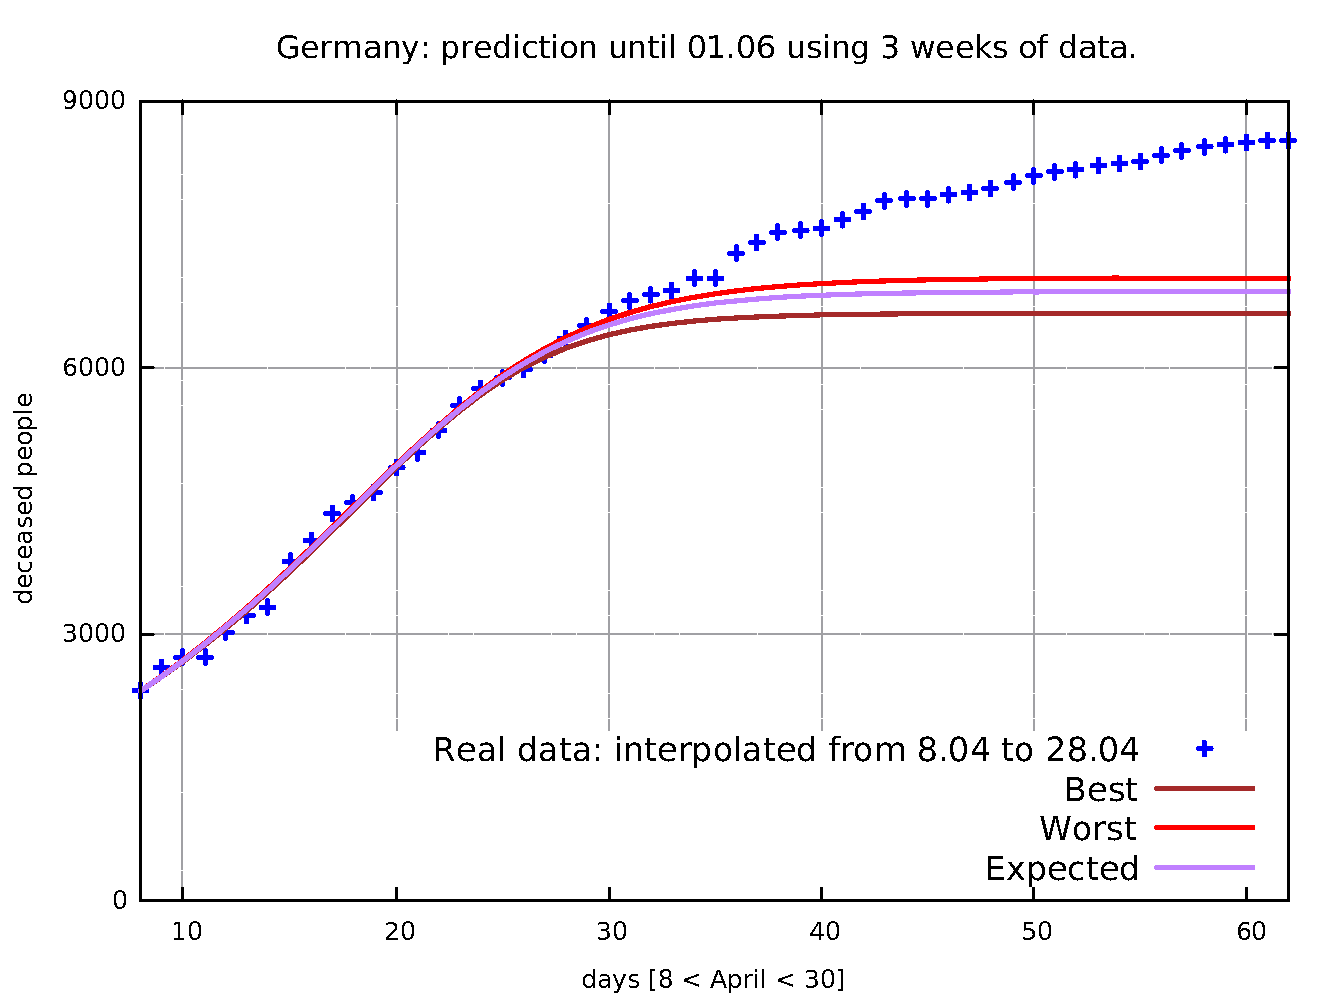
\includegraphics[width=\linewidth]{../../err10p_simulations/de/8-28/8-28.pdf}
	\end{figure}
\end{frame}


\begin{frame}
	\frametitle{Results: Italy, assuming $100\%$ of "error"}
	\begin{figure}
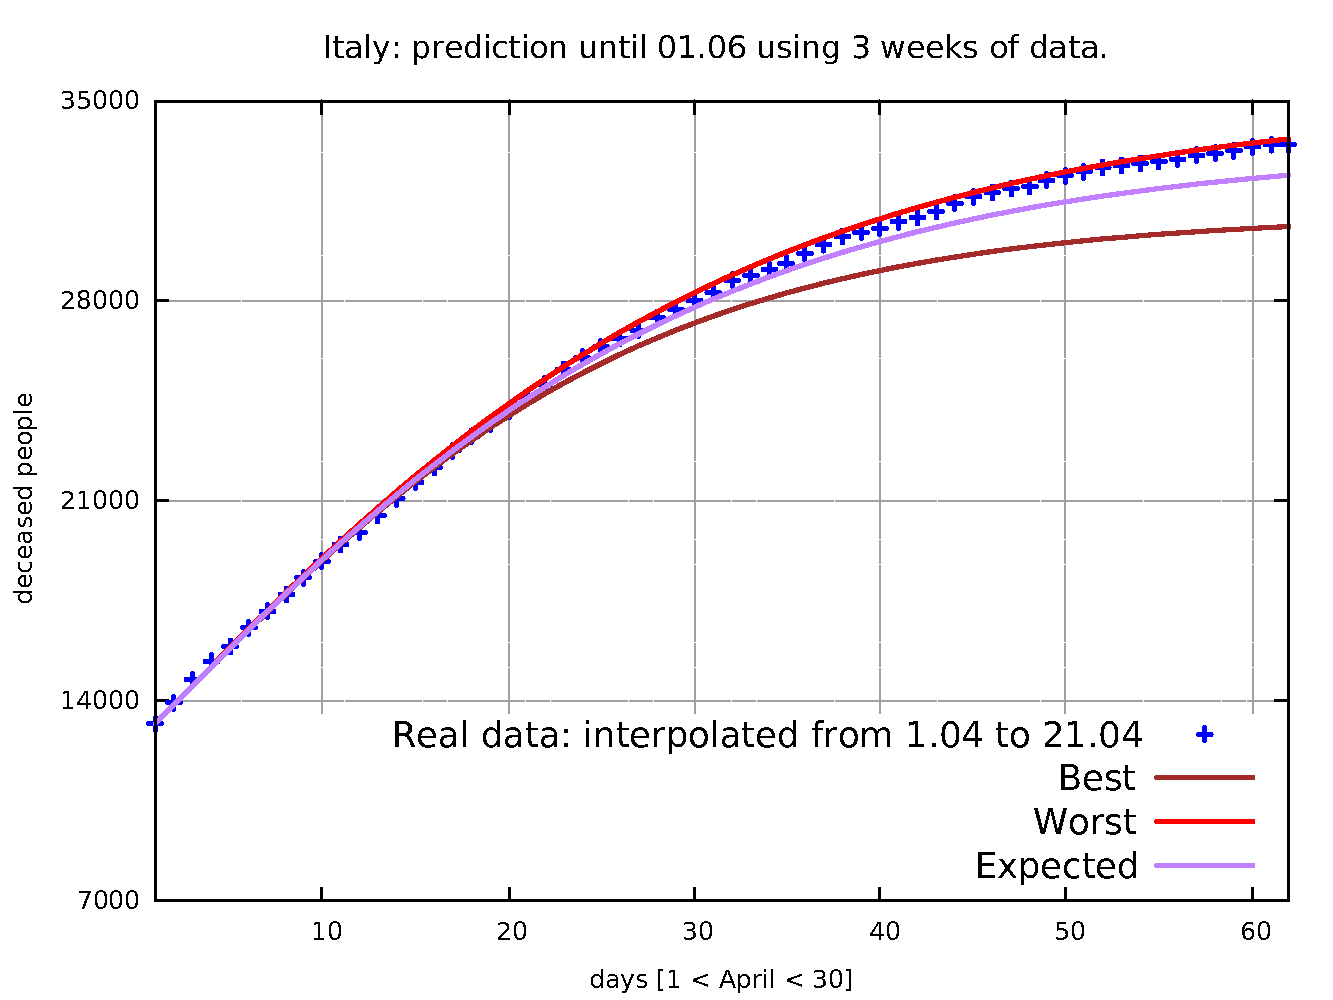
\includegraphics[width=\linewidth]{../../err100p_simulations/it/1-21/1-21.pdf}
	\end{figure}
\end{frame}

\begin{frame}
	\frametitle{Results: France, assuming $100\%$ of "error"}
	\begin{figure}
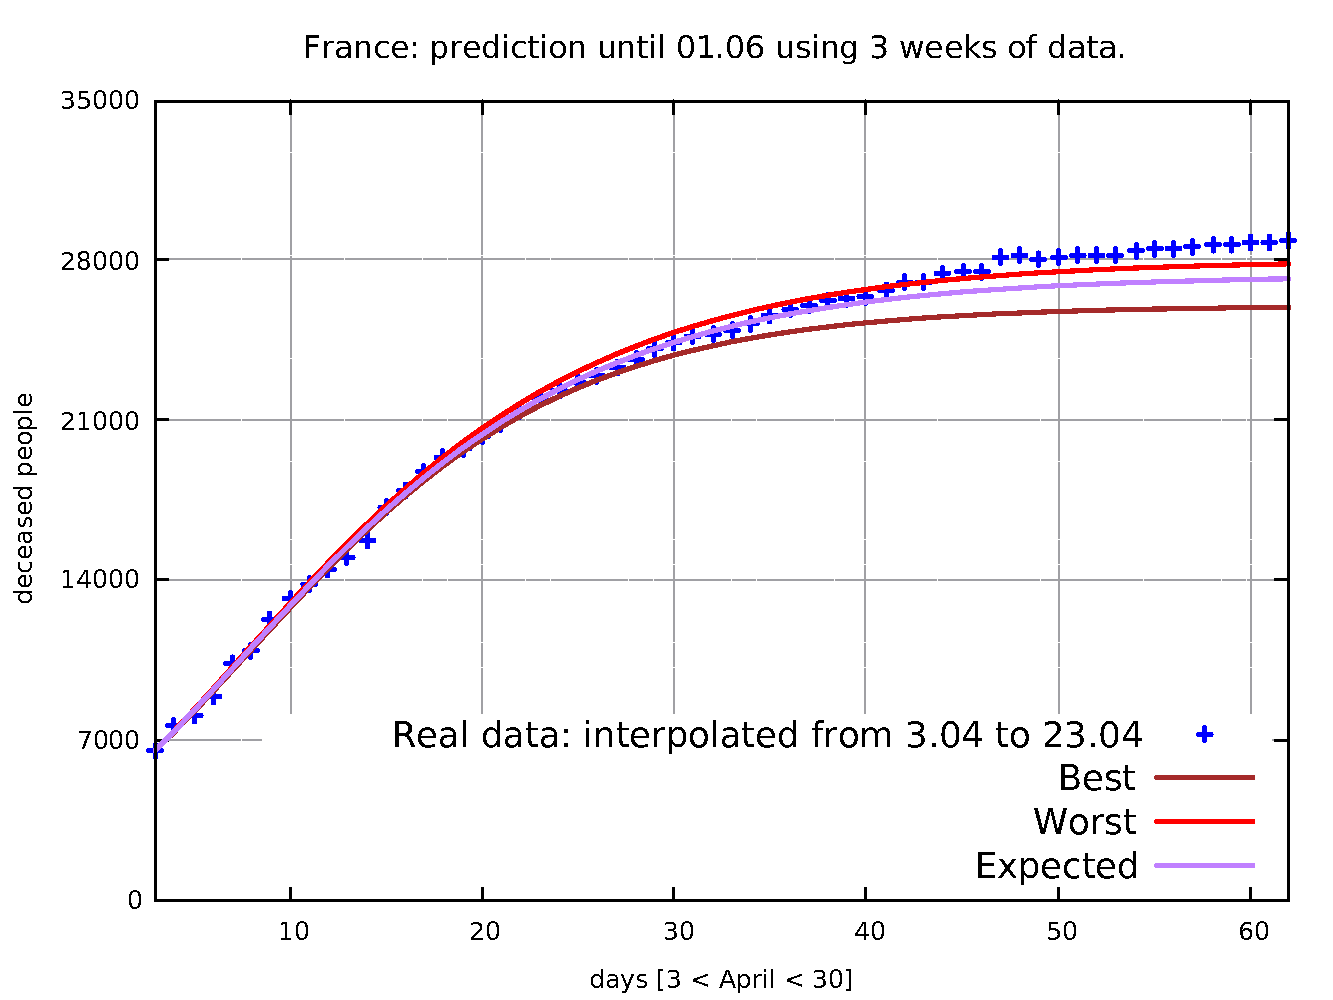
\includegraphics[width=\linewidth]{../../err100p_simulations/fr/3-23/3-23.pdf}
	\end{figure}
\end{frame}

\begin{frame}
	\frametitle{Results: Germany, assuming $100\%$ of "error"}
	\begin{figure}
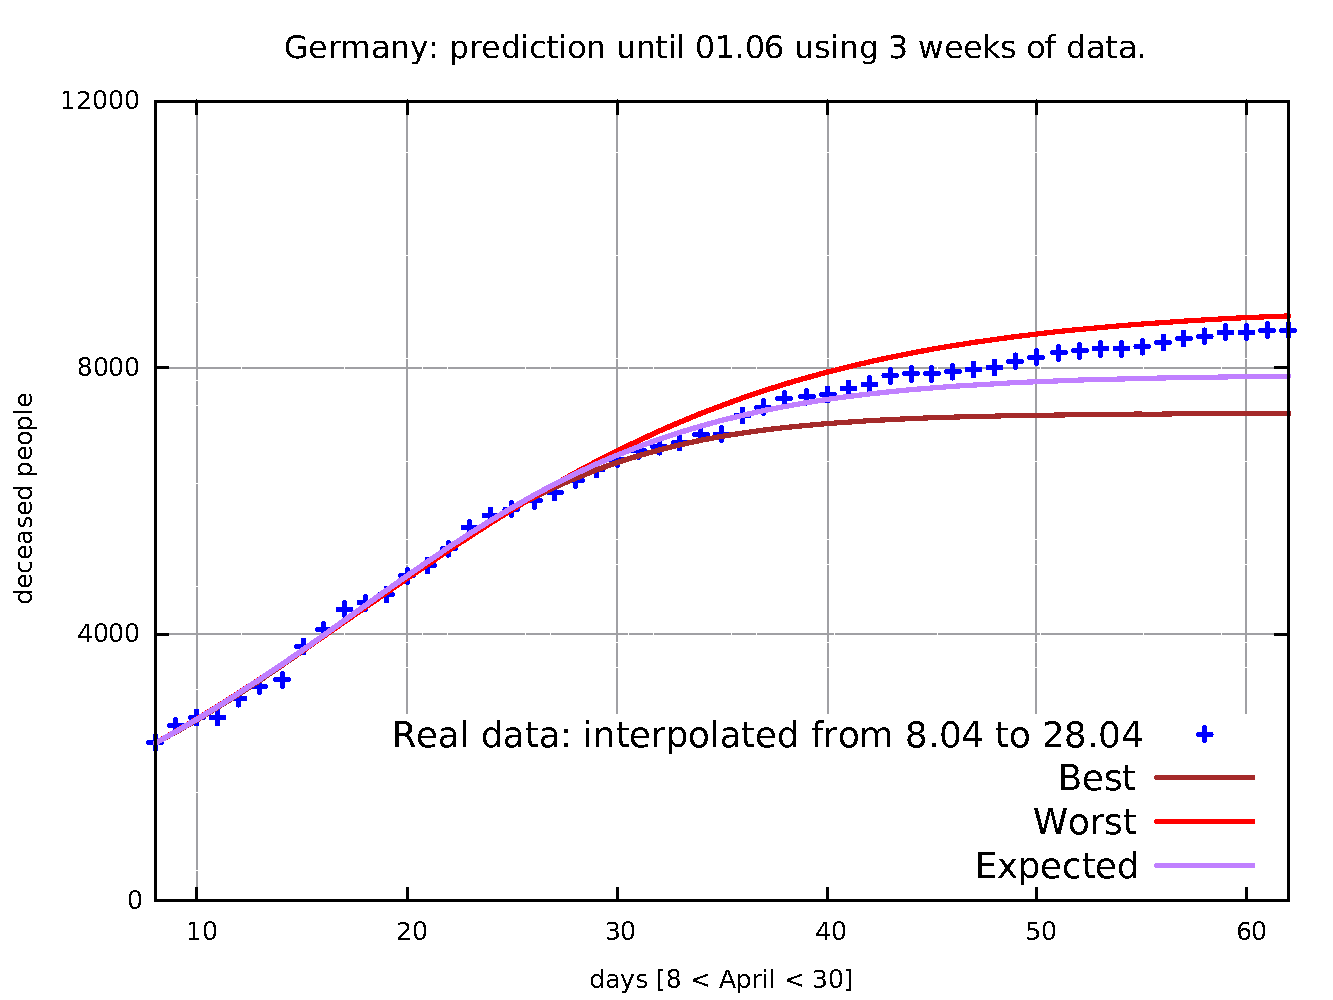
\includegraphics[width=\linewidth]{../../err100p_simulations/de/8-28/8-28.pdf}
	\end{figure}
\end{frame}

\begin{frame}
	\frametitle{Conclusions}
	Despite various theoretical issues, the results give some
	degree of satisfaction. \textcolor{red}
	{But they \emph{do not seem} to work
	with Spain, UK (I quickly tested)}.
	\begin{itemize}
		\item<1-> A next step can be to use the last 20 days of data
			to predict for June/July;
		\item<2-> Or try with another more appropriate Monte
			Carlo methods with better prior measures;
		\item<3-> Or instead of the Bayesian approach,
			try maximizing the Likelihood (i.e.
			probabilistic least square);
		\item<4-> Or simply to consider this example as a nice
			application of Monte Carlo Bayesian techniques,
			before moving back to the main PhD topic.
	\end{itemize}
\end{frame}

\begin{frame}
	Thanks for the attention!
\end{frame}

\end{document}
